The choice of rods to model the cable was done because it seemed to be the simpler
way to get a good cable behaviour.
\section{Rod Cable Model}

The present model is developed using the work by Vegar Johansen PhD thesis~\cite{johansen2007modelling} as a basis, in this model the rods are modelled by vectors and centres of gravity and allows the application of different forces on the cable, in this model the fluid friction is added.

A rod can characterised by the two following object:

\begin{align}
r &= \begin{bmatrix}
    r_x \\
    r_y \\
    r_z
\end{bmatrix}\, \textnormal{is the center of gravity}\\
b &= \begin{bmatrix}
    b_x \\
    b_y \\
    b_z
\end{bmatrix}\, \textnormal{is the vector for the rod orientation}
\end{align}

The forces acting on the cable are applied on the ends of each rods, meaning for example, the gravity force would be split in two forces acting on each side of the bar. Leading to the base formulas where a and c are the extremity of the bar ,  $f_X$ is the force applying at the point $X$ and $L$ is the length of the rod :

\begin{align}
\ddot{r} &= \dfrac{1}{m}  (f_a+f_c) \\
\ddot{b} &=  \dfrac{6}{m}(f_a+f_c) - \dfrac{b}{L^{2}}  (\dfrac{6}{m}b^{T}(f_a+f_c)+\dot{b}^{T}\dot{b}) 
\end{align}



Then the model adds the use of the Baumgarte stabilization constraint~\cite{baumgarte1972stabilization} to respect the physical constraint on the bar , length and position of fixed points if there is, thus changing the precedent equation. 
The stabilization technique is a PID method therefore it depends on coefficient parameters, in a variable-step solver augmenting the P an D coefficient improve the simulation but will increase the time needed to do the simulation.

Johansen proposes three scenarios for this model, a free cable, a fixed-free scenario where one side of the cable is attached to a point and the last one is a fixed-fixed where both side are attached to points.
The model interesting for the modelling of the sailboat towing a cable is the fixed-free scenario where the attachment point is the boat.

Applying force on each rod are the gravity, Archimedes principle and the fluid friction, for the rod $n$ :

{
\begin{align}
\centering
F_{fluid~n,a,x} &= -\frac{C_D (2 r ) \rho}{2} \cdot \displaystyle \int_{0}^{L/2} v_{a,x}(l)^2 \cdot \frac{2l}{L} \, \mathrm{d}l\ \nonumber \\
\vec{v_{a}}(l) &= \vec{\dot{r_n}} - \frac{2 l}{L} \cdot \vec{b_n} \times \frac{\vec{\dot{b_n}}}{L} \nonumber \\
\vec{v_{b}}(l) &= \vec{\dot{r_n}} + \frac{2 l}{L} \cdot \vec{b_n} \times \frac{\vec{\dot{b_n}}}{L}
\end{align}
}

The term $\frac{2 l }{L}$ in the integral part is to compensate the lever effect when applying this force on the extremity of the rod.



\begin{figure}[H]
\centering
    \begin{minipage}[b]{0.4\textwidth}
    \centering
    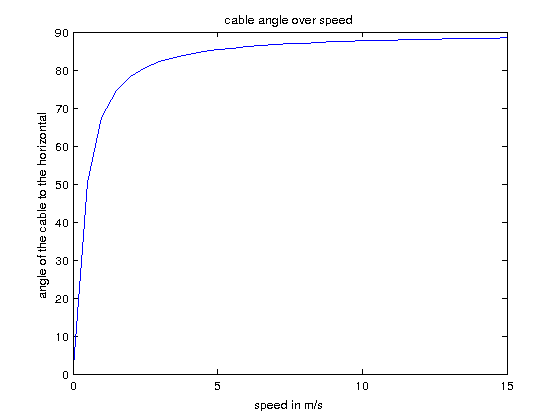
\includegraphics[scale=0.45,angle=0]{inde_cable_angle_speed.png}
    \caption{Angle of the cable when stabilized at the final speed.}
    \label{fig:angleIndSpeed}
    \end{minipage}
    \hfill
    \begin{minipage}[b]{0.45\textwidth}
    \centering
    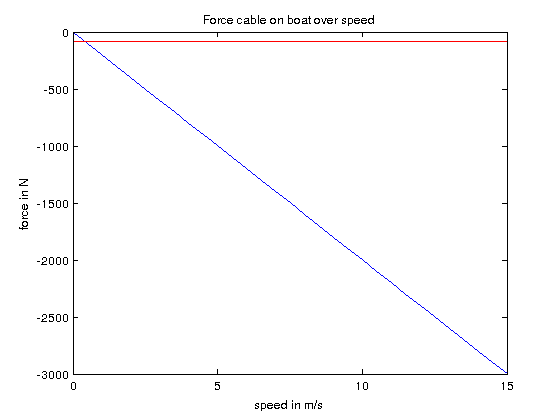
\includegraphics[scale=0.45,angle=0]{inde_cable_force_speed.png}
    \caption{Force of the cable on the boat when stabilized at the final speed.}
    \label{fig:forceIndSpeed}
    \end{minipage}
\end{figure}

By doing simulation with this model, the profile of the angle of the cable over speed is the same as in the Simulink model and the same can be done for the reaction of the cable on the boat, an constant for the vertical reaction and a linear decrease for the horizontal reaction dependant on the fluid friction force.

This model include a tolerance to errors which are resolved by the Baumgarte stabilisation technique but 
there still some left over:


\begin{figure}[H]
\centering
    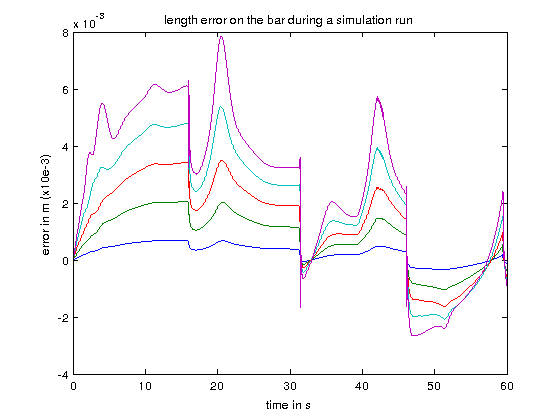
\includegraphics[scale=0.5,angle=0]{error_length_run.png}
    \caption{Error in length of the rods during a simulation run.}
    \label{fig:errorLRod}
\end{figure}

In the figure~\ref{fig:errorLRod} the error in length reach a maximum around one centimetre for a rod length of four meters\footnote{To see simulations : \href{https://www.youtube.com/watch?v=T7DRGq3E5x8}{Fixed cable video https://www.youtube.com/watch?v=T7DRGq3E5x8} or \href{https://www.youtube.com/watch?v=V4X0PsgsXZY}{Moving cable with a constant speed video https://www.youtube.com/watch?v=V4X0PsgsXZY}}, this error can be considered negligible in this case but in some runs if the start is too sharp then, the simulation may diverge.

In this model each rod can have a different length and mass:


\begin{figure}[H]
\centering
    \begin{minipage}[b]{0.4\textwidth}
    \centering
    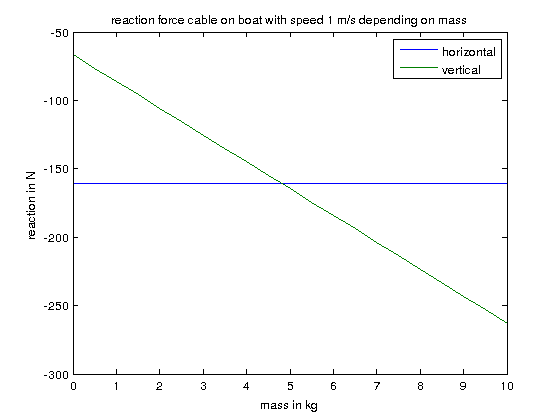
\includegraphics[scale=0.45,angle=0]{inde_cable_force_mass.png}
    \caption{Variation of reaction force of cable on boat depending on mass of last rod.}
    \label{fig:massForce}
    \end{minipage}
    \hfill
    \begin{minipage}[b]{0.45\textwidth}
    \centering
    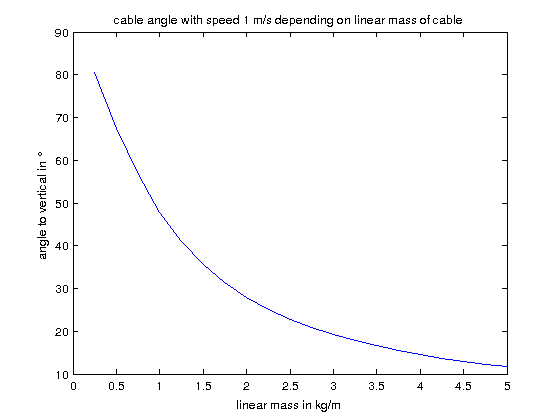
\includegraphics[scale=0.45,angle=0]{inde_cable_angle_linmass.png}
    \caption{Variation of the angle of the cable depending on the linear mass of the rods.}
    \label{fig:linmassAngle}
    \end{minipage}
\end{figure}

\begin{equation}
 \vec{0} = \vec{f}_{cable/boat}+\vec{f}_{fluid}+\vec{P}+\vec{\Pi}\\
 \label{equ_Stab}
\end{equation}

In figure~\ref{fig:massForce} is represented the force of the cable on the boat once stabilized and depending of the mass of the last rod. The horizontal force is constant over mass, this is logical as when stabilized mass does not appear in the horizontal part of the equation \eqref{equ_Stab}. And as for the vertical reaction it vary linearly with the mass,thus corresponding to the precedent equation on the z axis.

Changing the linear mass or the mass of the last rod have different effect on the final angle of the cable(see~\ref{fig:linmassAngle}).


To simulate this model there is more than one options, but to not make it diverge tweaking must be made.
If using a fixed-step size integration (Runge-Kutta) the step need to be $\sim\mathcal{O}(10^{-3})$, it is the limit of this method and if the cable endure big acceleration it will diverge.

With an solver with variable step-size (ODE45) the result will be in general more accurate but the computation time became very high needing more than one second to compute one second of simulation.If possible Matlab coder should be used to help improve the computation time.
